%\chapter{\normalsize{BACKGROUND OF SATELLITE REMOTE SENSING}}
\chapter{\normalsize{SATELLITE DATA ANALYSIS}}
%\section{Technique 5: Processing satellite data using GIS Software}
%\section{Objectives}
\paragraph{}
The main objective of this analysis is to process satellite data and compare with data obtained from aviation meteorolgical stations. Here we will use the three hour data from  \href{https://ldas.gsfc.nasa.gov/gldas}{GLDAS}.
\section{Aviation meteorological stations in cameroon}
\begin{table}[H]
\caption{Aviation meteorological stations}
\begin{figure}[H]
\begin{center}
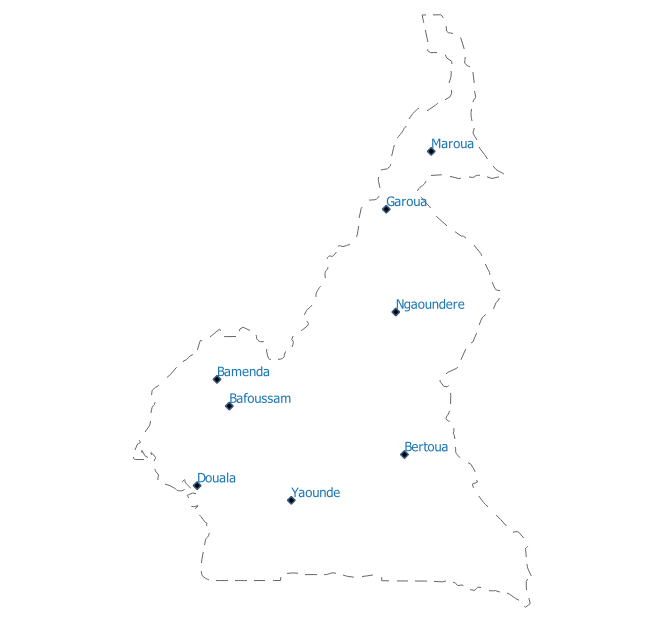
\includegraphics[scale=0.4]{cmr_station.png} %\cite{umhe}
\end{center}
\caption{aviation meteorological stations}
\label{aviation meteorological stations}%\cite{ABIA}
\end{figure}
\label{tab:Aviation meteorological stations}
\begin{center}
\begin{tabular}{| l | c | c | c | c |}
\hline
\textbf{\small{NAME}} & \textbf{\small{OMM CODE}} & \textbf{\small{ICAO CODE}} & \textbf{\small{LATITUDE}} & \textbf{\small{LONGITUDE}}\\[2pt] \hline
\small{Yaounde}	& \small{64950}&	\small{FKYS}&	\small{03°50’N}&	\small{011°31E} \\\hline
\small{Douala}	& \small{64910}	& \small{FKKD}	& \small{04°00’N}& 	\small{009°44’E} \\\hline
\small{Garoua}	& \small{64860}& 	\small{FKKR}& 	\small{09°20N}& 	\small{013°23’E}\\\hline
\small{Maroua}	& \small{64851}	& \small{FKKL}& 	\small{10°27’N}	& \small{14°15’E}\\\hline
\small{Bafoussam}& 	\small{64894}& 	\small{FKKU}& 	\small{05°32’05N}& 	\small{010°21’15E}\\\hline
\small{Bertoua}& 	\small{64930}& 	\small{FKKO}& 	\small{04°36’N}& 	\small{013°44’E}\\\hline
\small{Bamenda}& 	\small{64892}& 	\small{FKKV}& 	\small{06°03’N}& 	\small{010°07’E}\\\hline
\end{tabular}
\end{center}
\end{table}
\section{GLDAS data}
\paragraph{}
The goal of the Global Land Data Assimilation System (GLDAS) is to ingest satellite- and ground-based observational data products, using advanced land surface modeling and data assimilation techniques, in order to generate optimal fields of land surface states and fluxes (Rodell et al., 2004a).
GLDAS data are available to download from this \href{https://hydro1.gesdisc.eosdis.nasa.gov/data/GLDAS/GLDAS_NOAH025_3H.2.1/}{link}.
Detailed documentation about GLDAS 2.1 product is available \href{https://hydro1.gesdisc.eosdis.nasa.gov/data/GLDAS/GLDAS_NOAH025_3H.2.1/doc/README_GLDAS2.pdf.}{here}  
\section{Specific requirements}
\paragraph{}
The requirements for the metereorological data at aviation station are:
\begin{table}[H]
\caption{meteorological data required}
\label{tab:meteorological data required}
\begin{center}
\begin{tabular}{| l | c | c |}
\hline
\textbf{PARAMETER} & \textbf{SYMBOLS} & \textbf{UNIT}\\[2pt] \hline
Wind Speed & Ws&  m/s\\\hline
Air Temperature & Tair  & °C \\\hline
Pressure & P & hpa\\\hline
Relative Humidity & Rh  &   \% \\ \hline
\end{tabular}
\end{center}
\end{table}
\paragraph{}
The units at which GLDAS provide air temperature (K) and Pressure(Pa). Further GLDAS provide specific humidity. 
To match requirements the following conversion steps have to be performed:
\begin{description}
\item[Step 1] : Convert GLDAS air temperature from Kelvin to Deg C.
\item[Step 2] : Convert the unit of GLDAS pressure from Pa to Milli bar (Mb).
\item[Step 3] : Convert specific humidity to relative humidity following the description \href{https://earthscience.stackexchange.com/questions/2360/how-do-i-convert-specific-humidity-to-relative-humidity/}{here}.
\item[Step 4] : Extract the Ws, Tair, P and Rh corresponding at our aviation meteorological stations at observation time : 00:00, 03:00, 06:00, 09:00, 12:00, 15:00, 18:00 and 21:00 UTC.
\item[Step 5] : Compare the results with data collected at the stations.
\end{description}
\section{Download GLDAS data}
\paragraph{}
GLDAS documentation project provide python script to download data.
We run the script below to download data from 01 to 31 January 2021.
\begin{lstlisting}[language=Bash]
## In the Ubuntu session.
## Type in the following command to install the python package "gldas"
pip3 install gldas
## press enter
## Below code will download the GLDAS data between the dates provided in the command.
gldas_download -s 2021-01-01 -e 2021-01-31 --product GLDAS_Noah_v21_025 --username nina.younkap --password ****** /mnt/path/to/folder
## Note that the last argument in above command is path to a folder where the downloaded files will be stored.
\end{lstlisting}
\section{Processing single data file}
\subsection{ Data file structure}
\paragraph{}
Let us now see how to process a single NetCDF file (.\scriptsize{nc4} \normalsize)  dowloaded from GLDAS using the previous step and perform the required conversions.
For example let us consider the GLDAS data representing 06:00 hours on 31 January 2021.
The GLDAS file name follows a particular structure.
\newline
The file name is \scriptsize{GLDAS\_NOAH025\_3H.A20210131.0600.021.nc4} \normalsize
\begin{itemize}
\item \textbf{GLDAS\_NOAH025\_3H} represents the name, spatial resolution (025 means 0.25 degree resolution) and temporal resolution (3H means three hour data)
\item \textbf{A20210131}  represents the date of acquisition
\item \textbf{0600}  represents the time (in this case 06:00 GMT) the parameters are computed for.
\item \textbf{021}  represents the version of GLDAS data, in this case 2.1.
\item \textbf{nc4}  represents the extension and format of the data, in this case netCDF4.
\end{itemize}


\subsection{ Metadata discovery}
\paragraph{}
Now let us see how to read the metadata of this file in command line using gdal tools
\begin{lstlisting}[language=Bash]
## change directory to where you have downloaded the GLDAS data using the below
cd /mnt/d/mi_is_project_data/2021/31"
## Extract metadata of the 'GLDAS_NOAH025_3H.A20210131.0600.021.nc4' in the file "metadata.txt"
gdalinfo GLDAS_NOAH025_3H.A20210131.0600.021.nc4 > metadata.txt
## press enter
## Read metadata using vim editor
vim metadata.txt
\end{lstlisting}
\paragraph{}
In the metadata, under Subdatasets: all the parameters provided as subdatasets are listed. 
These subdataset names are used in the further steps to process individual parameters. For example, netCDF : \scriptsize{"GLDAS\_NOAH025\_3H.A20210131.0600.021.nc4" : Tair\_f\_inst} \normalsize is the name of air temperature grid at 06:00 on 31 January 2021 and we will use this name to extract/process this single grid. 
The codes of the parameters are listed in the \href{https://hydro1.gesdisc.eosdis.nasa.gov/data/GLDAS/GLDAS_NOAH025_3H.2.1/doc/README_GLDAS2.pdf}{GLDAS user manual} (Table 3.1).
\subsection{Single data extraction}
\paragraph{}
So for our project we need the following subdatasets from a single GLDAS file:
\newline
\vspace{0.5\baselineskip}
\scriptsize{NETCDF:"GLDAS\_NOAH025\_3H.A20210131.0600.021.nc4":Qair\_f\_inst} \normalsize- Specific humidity (Kg/Kg)
\newline
\vspace{0.5\baselineskip}
\scriptsize{NETCDF:"GLDAS\_NOAH025\_3H.A20210131.0600.021.nc4":Psurf\_f\_inst} \normalsize- Surface Pressure (Pa)
\newline
\vspace{0.5\baselineskip}
\scriptsize{NETCDF:"GLDAS\_NOAH025\_3H.A20210131.0600.021.nc4":Tair\_f\_inst} \normalsize - Air Temperature (K)
\newline
\vspace{0.5\baselineskip}
\scriptsize{NETCDF:"GLDAS\_NOAH025\_3H.A20210131.0600.021.nc4":Wind\_f\_inst } \normalsize - Wind speed (m/s)
\newline
\vspace{0.5\baselineskip}
\scriptsize{NETCDF:"GLDAS\_NOAH025\_3H.A20210131.0600.021.nc4":SWdown\_f\_inst} \normalsize - Downward short-wave radiation flux (W m-2)
\newline
Now let us extract each of the above subdatasets and convert them into tif file. For this we will use a gdal command called \scriptsize{gdal\_translate} \normalsize which is a global conversion tool for all kind of raster formats. 
\newline
Detailed documentation on \scriptsize{gdal\_translate} \normalsize is given \href{https://gdal.org/programs/gdal_translate.html}{here}.
\begin{lstlisting}[language=Bash]
##  Convert specific humidity to tif - below command
gdal_translate NETCDF:"GLDAS_NOAH025_3H.A20210131.0600.021.nc4":Qair_f_inst GLDAS_NOAH025_3H_A20210131_0600_Qair.tif
## Convert Surface Pressure to tif - below command
gdal_translate NETCDF:"GLDAS_NOAH025_3H.A20210131.0600.021.nc4":Psurf_f_inst GLDAS_NOAH025_3H_A20210131_0600_Psurf.tif
## Convert air temperature to tif - below command
gdal_translate NETCDF:"GLDAS_NOAH025_3H.A20210131.0600.021.nc4":Tair_f_inst GLDAS_NOAH025_3H_A20210131_0600_Tair.tif
## Convert Wind speed to tif - below command
gdal_translate NETCDF:"GLDAS_NOAH025_3H.A20210131.0600.021.nc4":Wind_f_inst GLDAS_NOAH025_3H_A20210131_0600_Wind.tif
## Convert Short wave downward radiation to tif - below command
gdal_translate NETCDF:"GLDAS_NOAH025_3H.A20210131.0600.021.nc4":SWdown_f_tavg GLDAS_NOAH025_3H_A20210131_0600_SWdown.tif
## Press enter
\end{lstlisting}
\newpage
\subsection{ Data visualisation in QGIS}
\paragraph{}
Now that we have the required parameters of 31 January 2021 in \scriptsize{.tif} \normalsize format, let us open the air temperature map in QGIS and see how it looks!
\begin{figure}[H]
\begin{center}
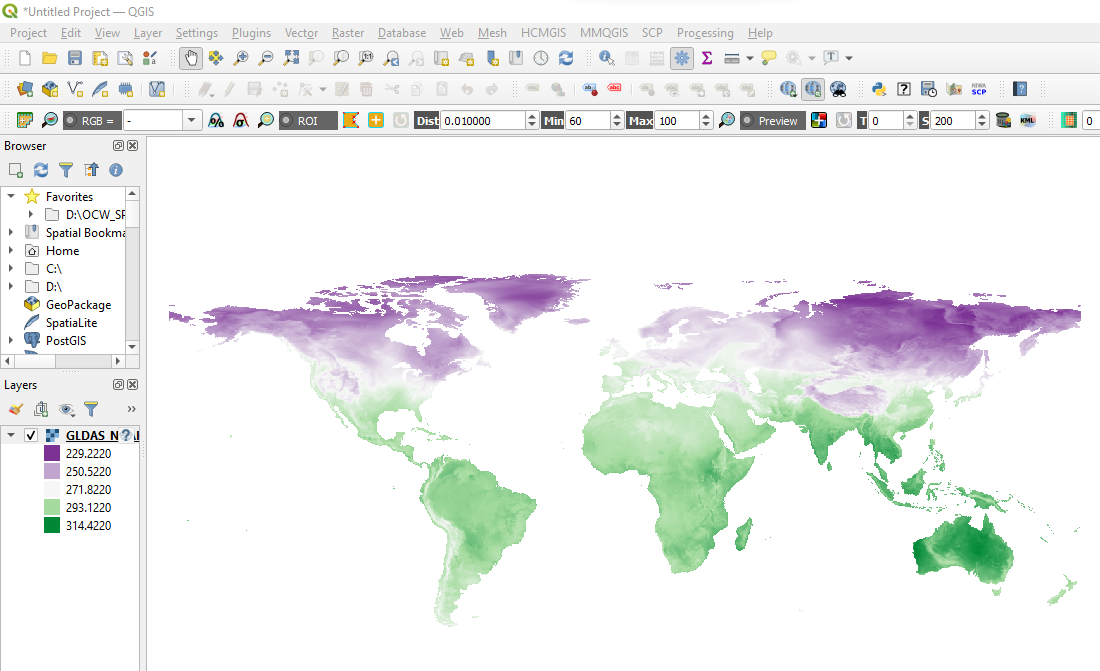
\includegraphics[scale=0.5]{qgis1.png} %\cite{umhe}
\end{center}
\caption{GLDAS Tair data displayed in QGIS}
\label{GLDAS Tair data displayed in QGIS}%\cite{ABIA}
\end{figure}
\paragraph{}
Let us also zoom to Cameroon boundaries and have a look at the Tair map.
\newline
Remember the resolution of data is 0.25 degrees.
\begin{figure}[H]
\begin{center}
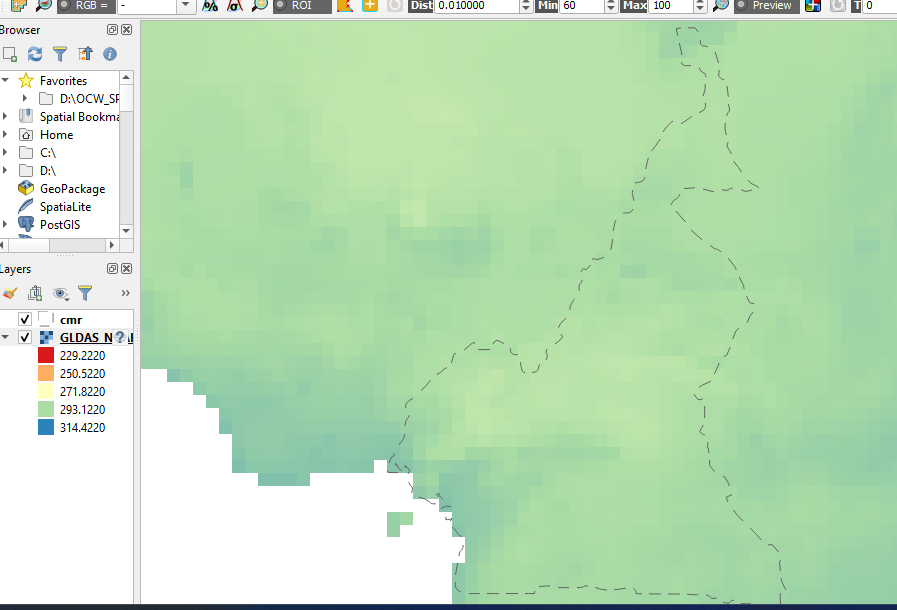
\includegraphics[scale=0.5]{qgis2.png} %\cite{umhe}
\end{center}
\caption{GLDAS Tair data displayed in QGIS and zoomed to Cameroon}
\label{GLDAS Tair data displayed in QGIS and zoomed to Cameroon}%\cite{ABIA}
\end{figure}
\subsection{ Unit data conversion}
\paragraph{}
Now let us see how to do unit conversion of all the four parameters required for aviation. 
One additional step is to clip the unit converted maps to cameroon boundaries as we are only interested in that region not global.
\newline
For further steps let us move to \textbf{GRASS GIS} as it is easier to do spatial and temporal analysis with GRASS library. 
We will create a new location and mapset for processing GLDAS data for Cameroon boundaries.
\begin{lstlisting}[language=Bash]
# Create (-c) just the location called "cmr" in epsg:4326 and exit (-e)
grass78 epsg:4326 /mnt/d/grassdata/cmr -c -e
# Create (-c) mapset called "met_data" inside the location "cmr" and open GRASS GIS in "cmr/met_data" mapset
grass78 /mnt/d/grassdata/cmr/met_data -c
# "-c" flag in above command is required only one time to create the mapset met_data
# Afterwards use below command to just start the existing mapset.
# grass78 /mnt/d/grassdata/cmr/met_data
\end{lstlisting}
\paragraph{}
Import the cameroon vector file , aviation meteorological station file , and others file required for our project into grass location. 
\begin{lstlisting}[language=Bash]
## IMPORT VECTOR DATA: Boundaries of Cameroon an  Aviation meteorological station in cameroon
## Navigate (cd) to the folder Cmr_Base_Layers
cd /mnt/d/mi_is_project_data/Cmr_Base_Layers 
# Import 'Cameroon' boundary shapefile into a vector in Grass GIS
v.import in=cmr.shp out=cmr
# Import 'Aviation meteorological staitions' points shapefile into a vector in Grass GIS
v.import in=aero_met_station_cmr.shp out=met_station
# Import 'FKKR TMA2' boundary shapefile into a vector in Grass GIS
v.import in=Fkkr_tma2.shp out=fkkr_tma2
# Import 'FKKN TMA' boundary shapefile into a vector in Grass GIS
v.import in=Fkkn_tma.shp out=fkkn_tma
# Import 'FKKL CONTROL ZONE' boundary shapefile into a vector in Grass GIS
v.import in=Fkkl_ctr.shp out=fkkl_ctr
# set the computational region to Cameroon Boundaries and set the computational resolution to 0.25 degrees
g.region vector=cmr res=0.25 -a
\end{lstlisting}
\newpage
\paragraph{}
To automate workflows, the following bash script process all the four required parameters (Tair, Rh, Wind speed and Psurf), clipped on cameroon boundaries  and converted to the required units from .nc4 files in a day.
\begin{lstlisting}[language=Bash]
#!/bin/bash
## This script process a single day GLDAS data and do all the required conversions needed for our project.
## GENERAL ##
if [ -z "$GISBASE" ] ; then
    echo "You must be in GRASS GIS to run this program." >&2
    exit 1
fi
# Set a environment to enable overwrite by default
export GRASS_OVERWRITE=1

# Navigate to the folder containing single day .nc4 files
#e.g INDAT="/mnt/d/mi_is_project_data/Cmr_Base_Layers/2021/01" for 01 January 2021
#Here we work on the  31 January 2021 data
INDAT="/mnt/d/mi_is_project_data/2021/031" 
cd ${INDAT}
# set the computational region to Urmia Lake basin and set the computational resolution to 0.25 degrees
g.region vector=cmr res=0.25 -a
# set the mask to cameroon boundaries

# For loop to process all the .nc files in one go
for i in `ls GLDAS*.nc4`; do
    dt=`echo ${i}|cut -d. -f2-3`
    #  Convert specific humidity to tif - below command
    gdal_translate NETCDF:"${i}":Qair_f_inst GLDAS_NOAH025_3H_${dt}_Qair.tif
    # Convert Surface Pressure to tif - below command
    gdal_translate NETCDF:"${i}":Psurf_f_inst GLDAS_NOAH025_3H_${dt}_Psurf.tif
    # Convert air temperature to tif - below command
    gdal_translate NETCDF:"${i}":Tair_f_inst GLDAS_NOAH025_3H_${dt}_Tair.tif
    # Convert Wind speed to tif - below command
    gdal_translate NETCDF:"${i}":Wind_f_inst GLDAS_NOAH025_3H_${dt}_Wind.tif
    # Convert Short wave downward radiation to tif - below command
    gdal_translate NETCDF:"${i}":SWdown_f_tavg GLDAS_NOAH025_3H_${dt}_SWdown.tif
    # Import to GRASS
    # Import and clip specific humidity
    r.import in=GLDAS_NOAH025_3H_${dt}_Qair.tif out=GLDAS_NOAH025_3H_${dt}_Qair -o
    # Import and clip Surface Pressure
    r.import in=GLDAS_NOAH025_3H_${dt}_Psurf.tif out=GLDAS_NOAH025_3H_${dt}_Psurf -o
    # Import and clip Tair
    r.import in=GLDAS_NOAH025_3H_${dt}_Tair.tif out=GLDAS_NOAH025_3H_${dt}_Tair -o
    # Import and clip Wind speed
    r.import in=GLDAS_NOAH025_3H_${dt}_Wind.tif out=GLDAS_NOAH025_3H_${dt}_Wind -o
    # Import and clip Short wave radiation
    r.import in=GLDAS_NOAH025_3H_${dt}_SWdown.tif out=GLDAS_NOAH025_3H_${dt}_SWdown -o
    # Unit conversion
    # Air temperature from Kelvin to degree celsius
    r.mapcalc "GLDAS_NOAH025_3H_${dt}_Tair_final = GLDAS_NOAH025_3H_${dt}_Tair - 273.15"
    # Short wave radiation (no conversion required)
    r.mapcalc "GLDAS_NOAH025_3H_${dt}_SWdown_final = GLDAS_NOAH025_3H_${dt}_SWdown"
    # Wind speed (no conversion required)
    r.mapcalc "GLDAS_NOAH025_3H_${dt}_Wind_final = GLDAS_NOAH025_3H_${dt}_Wind"
    ## Specific humidity re saved
    r.mapcalc "GLDAS_NOAH025_3H_${dt}_Qair_final = GLDAS_NOAH025_3H_${dt}_Qair"
    ## Pressure convert from pa to mb
    r.mapcalc "GLDAS_NOAH025_3H_${dt}_Psurf_final = GLDAS_NOAH025_3H_${dt}_Psurf / 100"
    ## Humidity according to the url: https://earthscience.stackexchange.com/questions/2360/how-do-i-convert-specific-humidity-to-relative-humidity
    r.mapcalc "es = 6.112 * exp((17.67 * GLDAS_NOAH025_3H_${dt}_Tair_final) / (GLDAS_NOAH025_3H_${dt}_Tair_final + 243.5))"
    r.mapcalc "e = (GLDAS_NOAH025_3H_${dt}_Qair_final * GLDAS_NOAH025_3H_${dt}_Psurf_final) / (0.378 * GLDAS_NOAH025_3H_${dt}_Qair_final + 0.622)"
    r.mapcalc "GLDAS_NOAH025_3H_${dt}_Rh = (e / es) * 100"
    # Final Relative humidity in %
    r.mapcalc "GLDAS_NOAH025_3H_${dt}_Rh_final = float(if(GLDAS_NOAH025_3H_${dt}_Rh > 100, 100, if(GLDAS_NOAH025_3H_${dt}_Rh < 0, 0, GLDAS_NOAH025_3H_${dt}_Rh)))"

done
\end{lstlisting}
\paragraph{}
We save the script above in the file \scriptsize{myscript.sh}.\normalsize The following code show how to run this file on Linux Operating System.
\begin{lstlisting}[language=Bash]
# Run the following command to install dos2unix
sudo apt-get install dos2unix
# Below command removes the trailing spaces from your script
dos2unix myscript.sh
# Run the following command to run the above saved script file
sh myscript.sh
# press enter
\end{lstlisting}
